\documentclass[11pt]{article}

\usepackage[utf8]{inputenc}
\usepackage[english]{babel}
\usepackage{hyperref}
\usepackage[toc,page]{appendix}

\usepackage{graphicx}
\usepackage{subcaption}

% Default fixed font does not support bold face
\DeclareFixedFont{\ttb}{T1}{txtt}{bx}{n}{12} % for bold
\DeclareFixedFont{\ttm}{T1}{txtt}{m}{n}{12}  % for normal

% Custom colors
\usepackage{color}
\definecolor{deepblue}{rgb}{0,0,0.5}
\definecolor{deepred}{rgb}{0.6,0,0}
\definecolor{deepgreen}{rgb}{0,0.5,0}

\usepackage{listings}
\lstset{
    language=python,
    basicstyle=\footnotesize\ttfamily,
    keywordstyle=\color{deepblue},
    emphstyle=\color{deepred},
    stringstyle=\color{deepgreen},
    frame=tb,
    showstringspaces=false
}

\usepackage[style=nature]{biblatex}
\addbibresource{references.bib}

\title{Search and Task Allocation \\
    \small{Game Theory}}

\author{Sebastian G. Winther-Larsen}

\begin{document}

    \maketitle

    \section{Introduction}
        This study is a continuation of a previous study where we 
        implemented a system of randomly moving reactive agents
        $R$ that solve tasks $T$ randomly distributed over 
        a square search area $A$~\cite{greg2020mas}. While we have 
        previously solved this search and task allocation (STA) problem
        with \emph{reactive}, passive agents; we will in this study solve the 
        same problem using \emph{strategic} agents.

        Now, whenever a new task is discovered an auction takes place among the 
        agents within communication range. The discoverer of the task functions 
        as the acutioneer, and the agents within communication distance as
        bidders. The potentially helping bidders use the distance to the 
        task as their bid in the auction. The acutioneer will recruit help 
        based on their bids in order to have enough agengs, including itself,
        to solve the task.

    \section{Extending PyGame Framework}

        From before we already have a framework implemented in PyGame\cite{pygame},
        that is able to simulate the STA problem with reactive agents. The 
        framework consists of three main classes, \lstinline|Agent|, \lstinline|Task|
        and \lstinline|Simulation|. The \lstinline|Task| class' relevant members
        are the task capacity $T_c$ and an \lstinline|update()| method that kills the 
        task if enough agents, compared to $T_c$, are tasked to it. The \lstinline|Agent|
        class' most important functionality is the \lstinline|update()| method that 
        functions differently depding on the \emph{state} of the agent. An agent can be 
        \emph{searching}, \emph{tasked} or \emph{called}. As such, it is a very passive 
        sprite. All other mechanics within the simulation is controlled by the 
        \lstinline|Simulation| class. Therefore, it is easiest from an implementation 
        standpoint to extend the \lstinline|Simulation| class to make the 
        agents strategic, because it is here that the states of the \lstinline|Agent| 
        class instances are changed.

        To accomplish this, we move the lines of code that checks if a task is 
        disovered, i.e. an agent is within task radius $T_r$ of the tasks, to a
        separate method within the \lstinline|Simulation| class. Then we can 
        create a subclass \lstinline|AuctionSimulation| that only needs to 
        reimplement this method, \lstinline|check_for_tasks()|. The entire implementation is 
        included in \autoref{app:code}.

    \section{Results}

        We perform five strategic agent simulations over $T=1000$ time steps for 
        different communication distances $R_d\in\{0, 100, 200, 300, 400, 600, 1000, 1400\}$.
        Figures showing cumulative number of tasks solved for these simulations are 
        provided in \autoref{app:figs}.

        A comparison of the strategic and reactive agents is shown in \autoref{fig:perf_compare}.
        We uncover no significant difference in performance between the two types of 
        agents for a low communication distance $R_d\leq600$. Above this level, the strategic
        agents perform significantly better.

        \begin{figure}
            \centering
            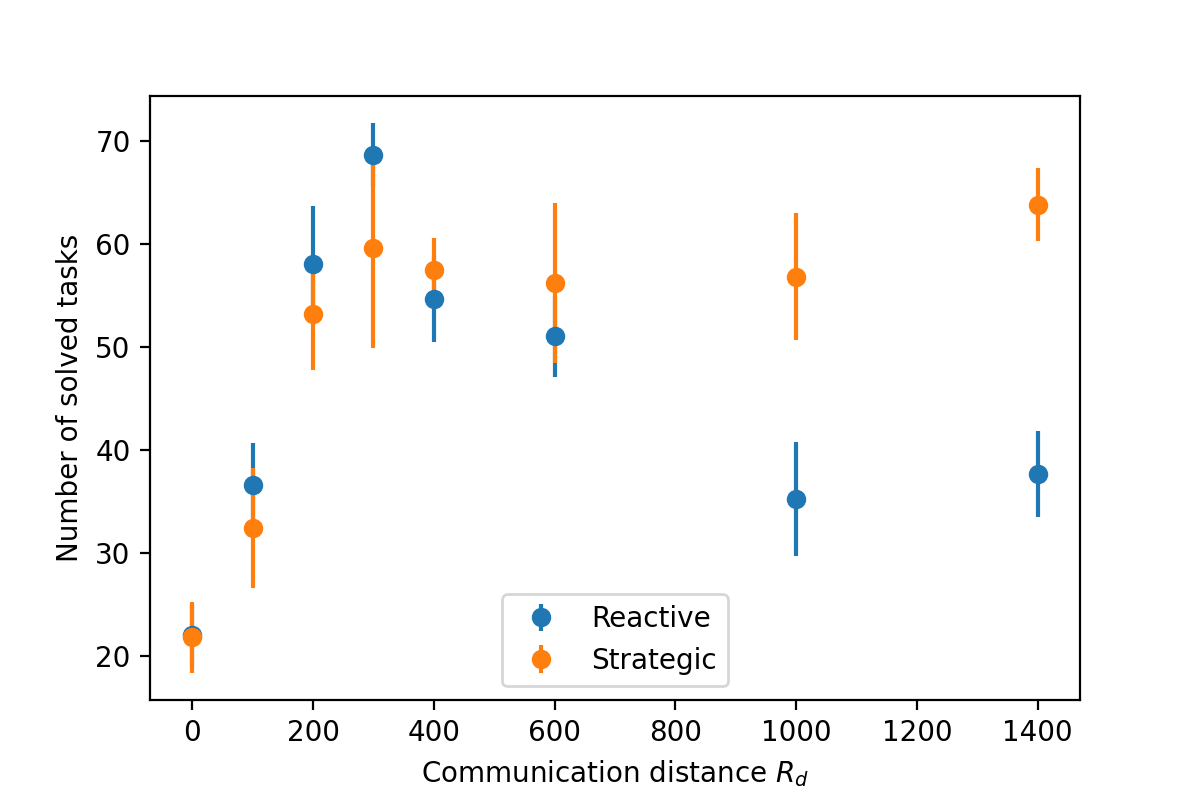
\includegraphics[width=0.8\textwidth]{figures/perf_compare.png}
            \caption{
                Comparison of strategic and reactive agents. Each point represents 
                the mean and standard deviation for number of solved tasks
                after $T=1000$ times steps for 
                five simulations. We notice a reduction in performance as the 
                communication distance $R_d$ increases for the reactive agents.
                \label{fig:perf_compare} 
            }
        \end{figure}


    \section{Discussion}

        The reason for the drop in performance for a long communication distance when 
        one is applying reactive agents is illustrated clearly in \autoref{fig:reactive_clustering}.
        When an agent discovers a task, a very large percentage of the other agents are called to its
        location, if the commucation radius $R_d$ reaches across a large part of the search area. This 
        in turn will sometimes result in clustering of agents, which again leads to a longer time until 
        the next task is discovered.

        \begin{figure}
            \centering
            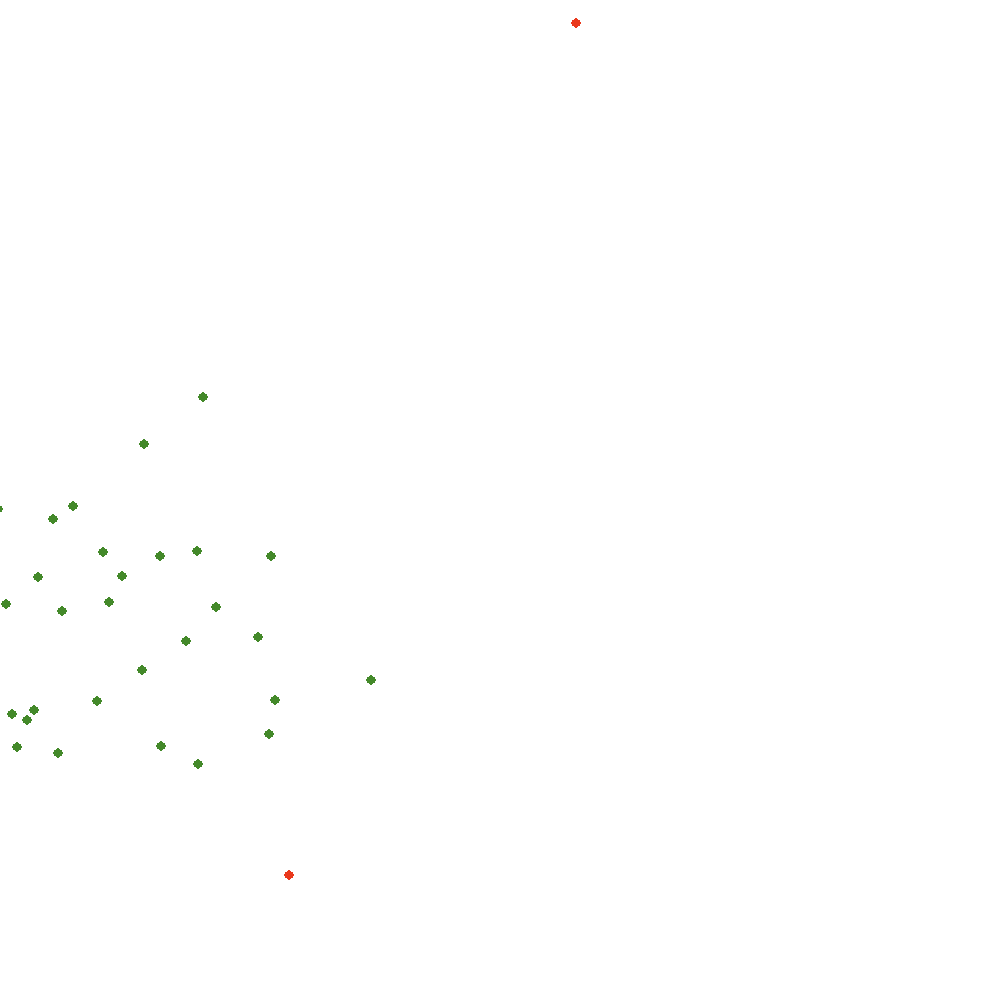
\includegraphics[width=0.8\textwidth]{figures/screenshot.png}
            \caption{
                Clustering of reactive agents that commonly occurs for high communication 
                distances - this is for $R_d = 1400$.
                \label{fig:reactive_clustering}
            }
        \end{figure}

        Several factors must be taken into account in the choice of agents. We assume here that strategic agents 
        are about twice as costly as reactive agents. The first thing to consider is what is known about the 
        search area. If one has knowledge of the size of the search area $A$, one can tune the communication 
        distance $R_d$ to be around half of the width of $A$, and reactive agents would perform just as well as 
        strategic agents. If one does not have this knowledge, one would 
        most likely be intersted in setting $R_d$ as high as possible, to make sure that agents can communicate at 
        all. Such a decision bears the risk of making the reactive agents preform at a suboptimal level.
        The difference in performance
        as shown in \autoref{fig:perf_compare} is $~25$ solved tasks for $R_d>1000$ after $T=1000$ time 
        steps. Since the cummulative number of solved tasks as a function of time appear to be linear,
        one would expect this difference to increase over time. Therefore, the time it takes to complete 
        the problem will affect the perfomance, favourably for strategic agents. After enough time, this 
        difference would quickly make up the difference in cost of agents. In conclusion, if it is possible
        to adjust the communication distance $R_d$ from prior knowledge of the search area $A$; use cheap,
        reactive agents. If the search area is unknown, opting for more dear strategic agents set with 
        very high $R_d$ is the prudent choice.

\printbibliography

\pagebreak
\appendix

\section{Figures}
\label{app:figs}

\begin{figure}[ht]
    \begin{subfigure}{.5\textwidth}
      \centering
      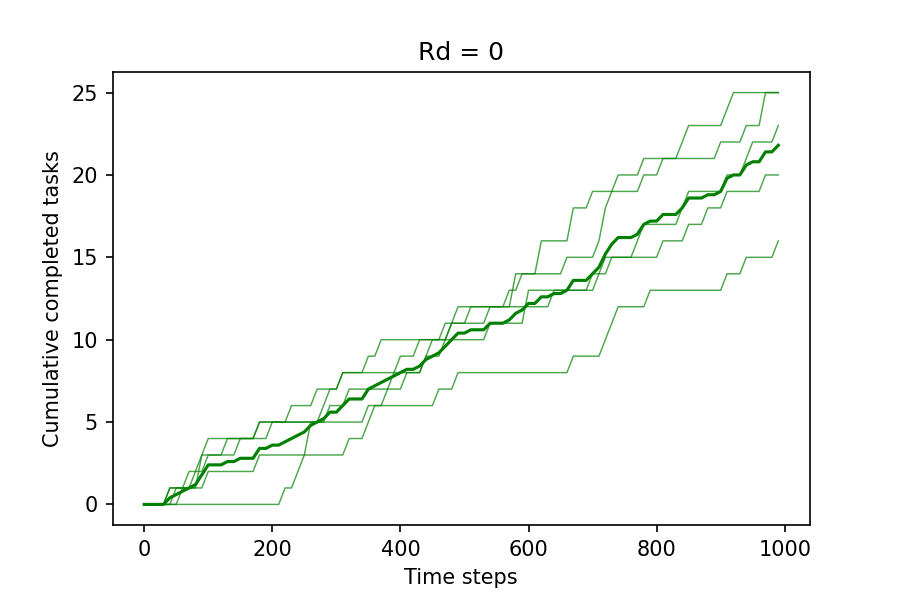
\includegraphics[width=\linewidth]{figures/Rd_0.png}
    \end{subfigure}
    \begin{subfigure}{.5\textwidth}
      \centering
      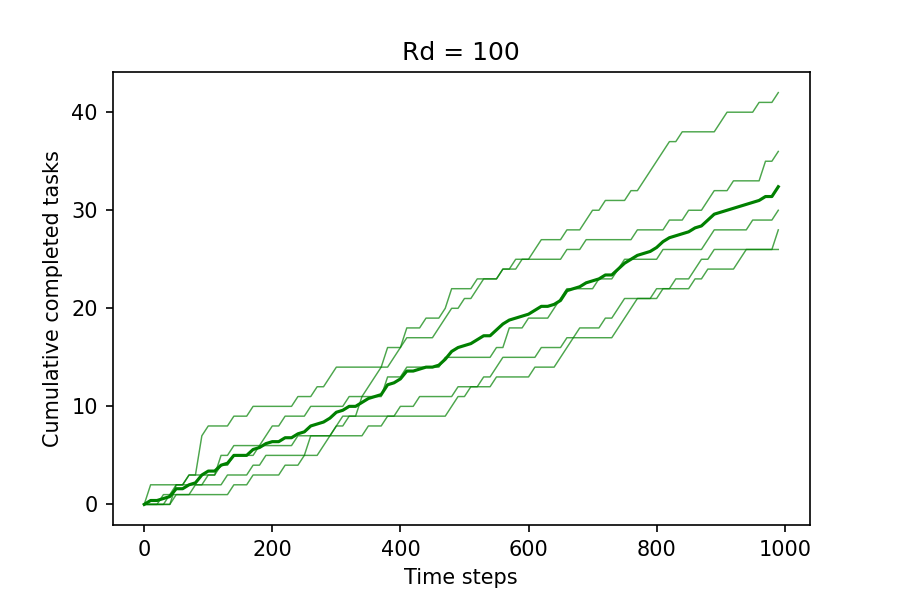
\includegraphics[width=\linewidth]{figures/Rd_100.png}
    \end{subfigure}
\end{figure}

\begin{figure}[ht]
    \begin{subfigure}{.5\textwidth}
      \centering
      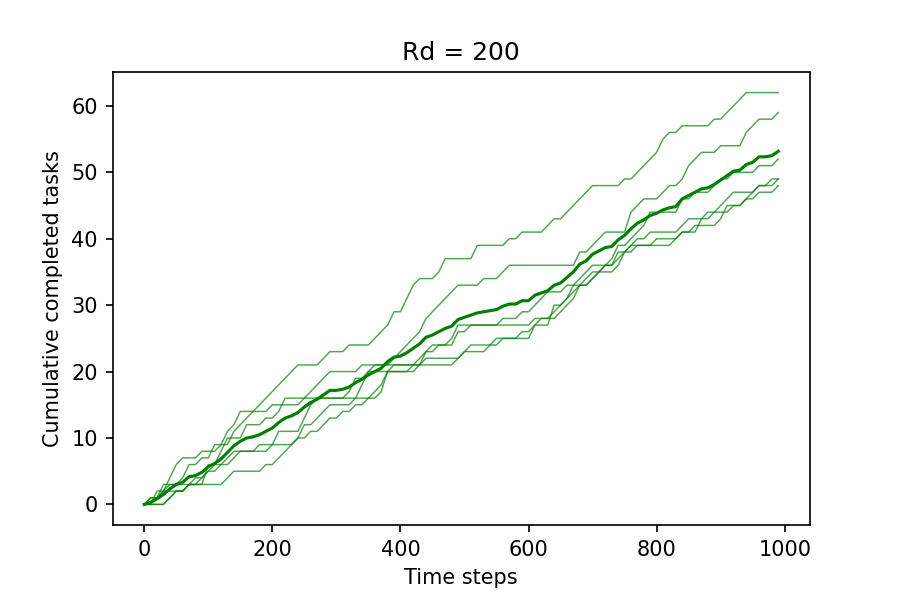
\includegraphics[width=\linewidth]{figures/Rd_200.png}
    \end{subfigure}
    \begin{subfigure}{.5\textwidth}
      \centering
      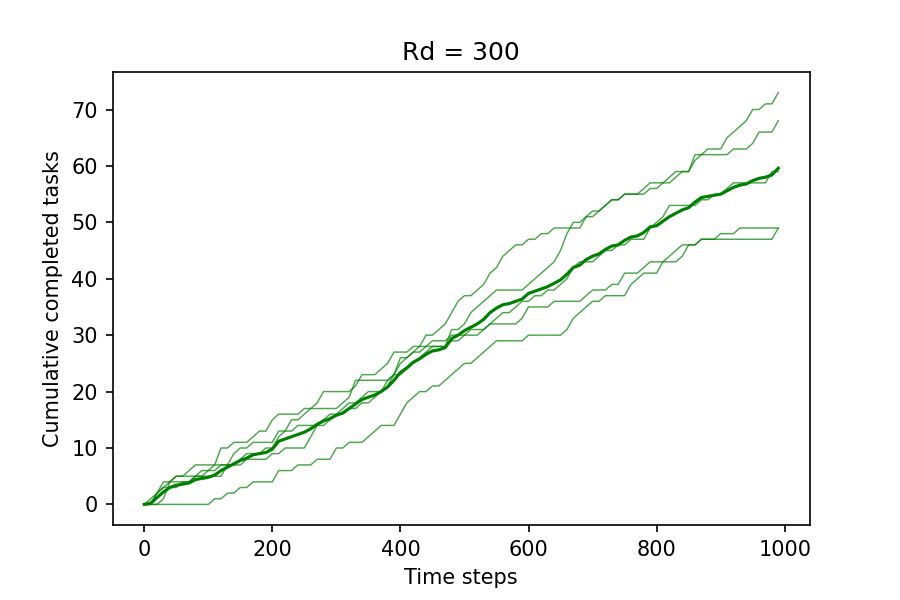
\includegraphics[width=\linewidth]{figures/Rd_300.png}
    \end{subfigure}
\end{figure}

\begin{figure}[ht]
    \begin{subfigure}{.5\textwidth}
      \centering
      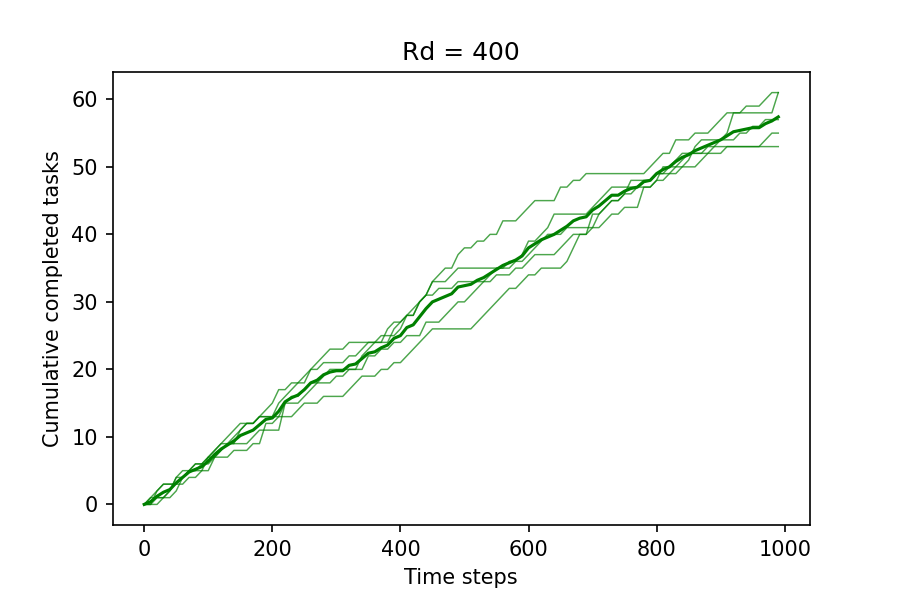
\includegraphics[width=\linewidth]{figures/Rd_400.png}
    \end{subfigure}
    \begin{subfigure}{.5\textwidth}
      \centering
      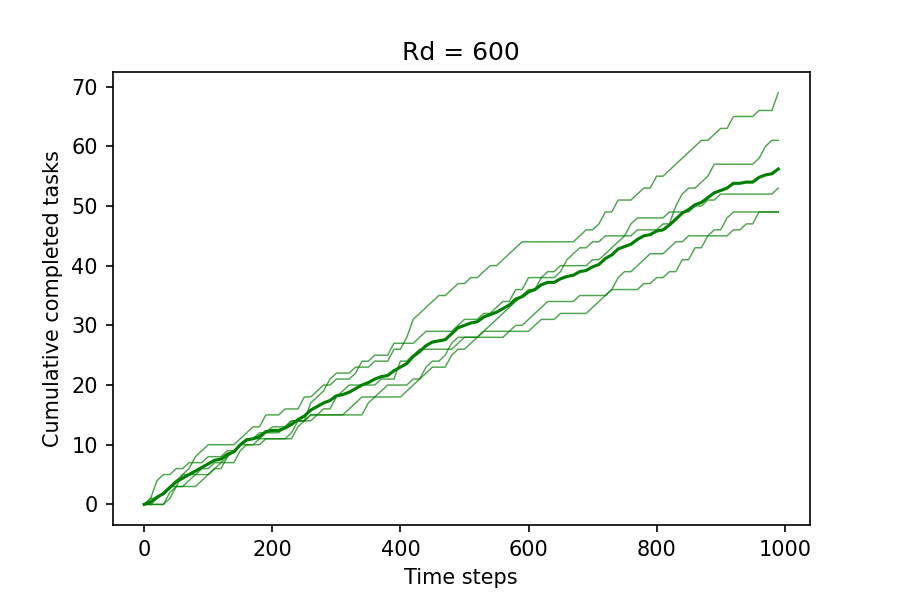
\includegraphics[width=\linewidth]{figures/Rd_600.png}
    \end{subfigure}
\end{figure}

\begin{figure}[ht]
    \begin{subfigure}{.5\textwidth}
      \centering
      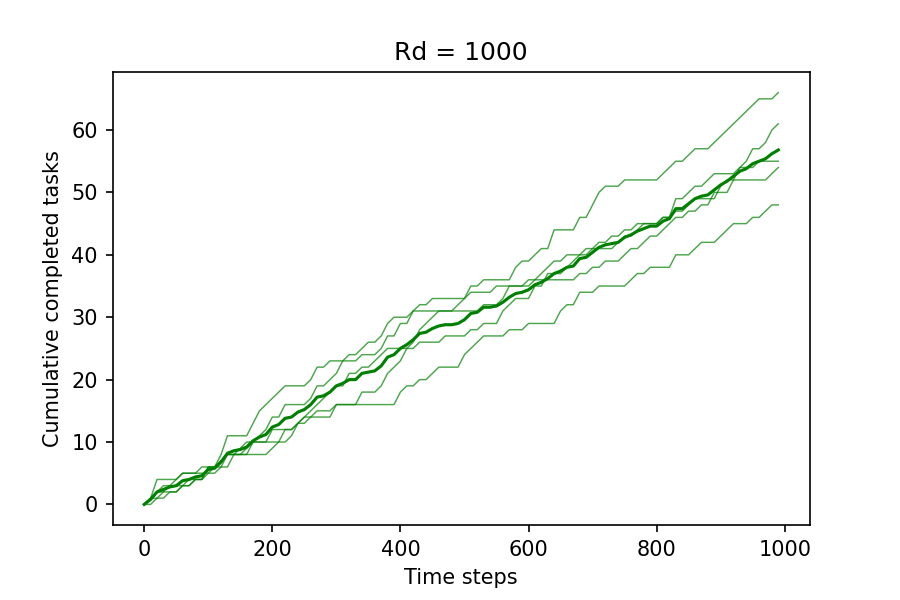
\includegraphics[width=\linewidth]{figures/Rd_1000.png}
    \end{subfigure}
    \begin{subfigure}{.5\textwidth}
      \centering
      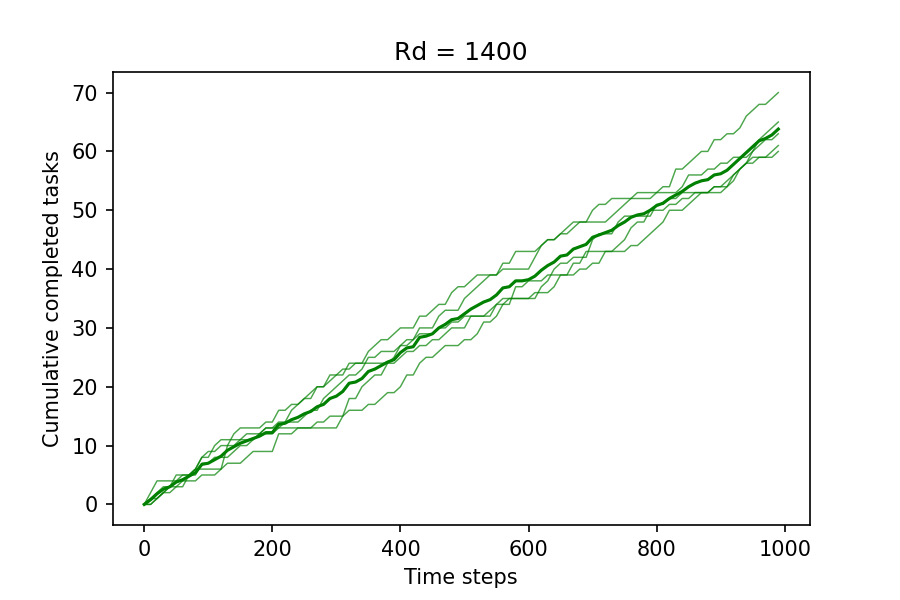
\includegraphics[width=\linewidth]{figures/Rd_1400.png}
    \end{subfigure}
\end{figure}

\pagebreak
\section{Code listing}
\label{app:code}

\lstinputlisting[firstline=0,lastline=280]{../pygame_task_search.py}

\end{document}